%% MoCafe v2.00 -- MPI Scaling Benchmark
%% Author: Kwang-Il Seon (KASI)
\documentclass[english,a4paper]{kiseon_memo}
\synctex=1

\usepackage{booktabs}
\usepackage{amsmath}
\usepackage{graphicx}
\usepackage{microtype}

\newcommand{\code}[1]{\texttt{#1}}
\newcommand{\file}[1]{\texttt{#1}}
\newcommand{\pp}[1]{\texttt{par\%#1}}
\newcommand{\Np}{N_{\rm p}}

\begin{document}

\title{MoCafe v2.00 --- MPI Scaling Benchmark}
\author{Kwang-Il Seon (KASI)}
\date{2026-07-11}
\maketitle

\begin{abstract}
\noindent
Strong- and weak-scaling measurements of MoCafe's MPI parallelization on a
dual-socket Xeon node, comparing the two photon-distribution modes
(\pp{use\_master\_slave} on/off).  Equal-share mode scales nearly ideally up to
the physical core count (94\% parallel efficiency at 16 ranks, 84\% at 32);
beyond the 36 physical cores hyper-threading adds little.  Master--slave mode
pays exactly one rank---the dispatcher---and nothing more: its runtime follows
the $(\Np-1)/\Np$ worker limit to within a few percent, so the two modes
converge above ${\sim}16$ ranks, and under hyper-threaded contention the
dynamic balancing of master--slave even wins slightly.  Recommendations: use
all physical cores but not the hyper-threads for production runs; at small
$\Np$ prefer equal-share unless the photon cost is strongly nonuniform.
\end{abstract}

\tableofcontents
\clearpage

%=============================================================================
\section{Setup}
%=============================================================================

\subsection{Hardware and software}
\begin{itemize}
\item Node: dual-socket Intel Xeon Gold 6254 @ 3.10\,GHz,
      $2\times18 = 36$ physical cores, 72 hardware threads (hyper-threading).
\item Compiler / MPI: Intel oneAPI \code{mpiifort} (\code{-ipo -O3 -no-prec-div
      -fp-model fast=2}), Intel MPI; one MPI rank per process, no OpenMP.
\item The node was otherwise idle (load ${\lesssim}1.5/72$) during the runs.
\end{itemize}

\subsection{Benchmark case}
A representative panchromatic transport run whose cost is dominated by the
photon loop (input \file{scale\_base.in} under \file{examples/scaling/}):
\begin{itemize}
\item SED mode (\pp{use\_sed}) with 40 log-spaced wavelength bins
      (0.0912--2000\,$\mu$m), astrodust opacities;
\item point source ($T_\star = 10^4$\,K) in a $\tau_V = 10$ dust sphere on a
      $33^3$ Cartesian grid;
\item the $J_\lambda$ path-length tally (\pp{save\_jlam}) active, so the
      measurement includes the per-rank tally and its final
      \code{MPI\_ALLREDUCE} ($40\times33^3 \approx 1.4$\,M doubles
      ${\approx}11$\,MB --- negligible here);
\item one small observer image ($33^2$); no dust-emission stage.
\end{itemize}
Timings are wall-clock times of the whole \code{mpirun} invocation, which
include a fixed ${\approx}0.9$\,s of startup (MPI init, opacity tables, grid).
Every run uses the same seed; the RNG streams differ per rank, so the physics
output is statistically, not bitwise, identical between the two modes.

\subsection{Protocol}
\begin{itemize}
\item \textbf{Strong scaling}: fixed $6.4\times10^{7}$ photons;
      $\Np = 1,2,4,\dots,64$ for equal-share and $\Np = 2,4,\dots,64$ for
      master--slave (a single rank cannot run master--slave: rank~0 only
      dispatches).
\item \textbf{Weak scaling}: $10^{6}$ photons per rank
      ($10^6\,\Np$ in total), same $\Np$ series.
\item Driver: \file{examples/scaling/run\_scaling.sh}; analysis:
      \file{plot\_scaling.py}; raw data: \file{results.csv}.
\end{itemize}

\subsection{The two distribution modes}
\begin{description}
\item[Equal share (\pp{use\_master\_slave} = .false.)]  Rank $r$ processes the
  photon indices $r{+}1, r{+}1{+}\Np, r{+}1{+}2\Np,\dots$  All $\Np$ ranks
  compute; there is no communication during the loop.  Load balance relies on
  photons having statistically similar cost.
\item[Master--slave (\pp{use\_master\_slave} = .true., default)]  Rank~0 hands
  out batches of \pp{num\_send\_at\_once} ($=10^4$) photons on demand and does
  not itself transport photons; the $\Np{-}1$ workers request a new batch when
  they finish one.  This buys dynamic load balancing at the cost of one rank,
  so its ideal runtime is $T_1/(\Np{-}1)$ rather than $T_1/\Np$.
\end{description}

%=============================================================================
\section{Strong scaling}
%=============================================================================

Table~\ref{tab:strong} lists the measured wall times; Fig.~\ref{fig:strong}
shows the speed-up and parallel efficiency, both relative to the single-rank
equal-share time $T_1 = 829.7$\,s.

\begin{table}[htb]
\centering
\caption{Strong scaling: $6.4\times10^{7}$ photons, wall time $T$ [s], speed-up
$S = T_1/T$, and parallel efficiency $E = S/\Np$.}
\label{tab:strong}
\begin{tabular}{r rrr rrr}
\toprule
      & \multicolumn{3}{c}{equal share} & \multicolumn{3}{c}{master--slave}\\
\cmidrule(lr){2-4}\cmidrule(lr){5-7}
$\Np$ & $T$ [s] & $S$ & $E$ [\%] & $T$ [s] & $S$ & $E$ [\%]\\
\midrule
  1 &  829.7 &  1.00 & 100.0 &    --  &   --  &  --  \\
  2 &  418.6 &  1.98 &  99.1 &  846.5 &  0.98 & 49.0 \\
  4 &  215.9 &  3.84 &  96.1 &  283.2 &  2.93 & 73.3 \\
  8 &  109.2 &  7.60 &  95.0 &  122.1 &  6.79 & 84.9 \\
 16 &   55.3 & 14.99 &  93.7 &   58.1 & 14.28 & 89.3 \\
 32 &   31.0 & 26.78 &  83.7 &   31.8 & 26.12 & 81.6 \\
 64 &   29.4 & 28.20 &  44.1 &   27.6 & 30.01 & 46.9 \\
\bottomrule
\end{tabular}
\end{table}

\begin{figure}[htb]
\centering
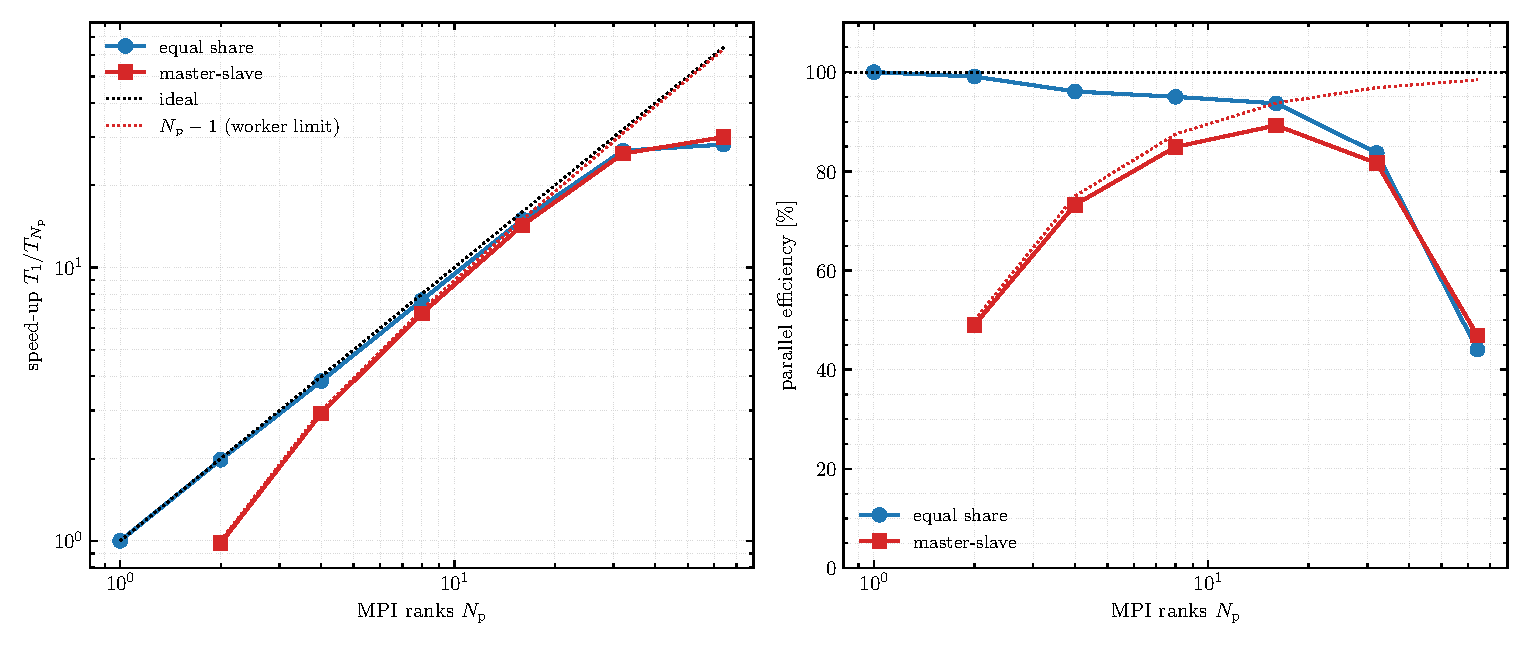
\includegraphics[width=\textwidth]{../examples/scaling/scaling_strong.pdf}
\caption{Strong scaling.  \emph{Left}: speed-up versus rank count with the
ideal line and the master--slave worker limit $S = \Np-1$.  \emph{Right}:
parallel efficiency; the red dotted curve is the worker-limit prediction
$100\,(\Np-1)/\Np$.  Both modes drop sharply at $\Np = 64$, which exceeds the
36 physical cores of the node (hyper-threading).}
\label{fig:strong}
\end{figure}

\subsection{Equal share}
The photon loop is communication-free, and the efficiency stays at
94--99\% up to $\Np = 16$ and 84\% at $\Np = 32$.  The mild decline toward 32
ranks is a hardware effect (shared caches and memory bandwidth on the two
sockets), not MPI overhead: the weak-scaling runs (\S\ref{sec:weak}) show the
same decline at constant communication volume.

\subsection{Master--slave: the cost is exactly one rank}
The master--slave times follow the worker limit $T_1/(\Np-1)$ closely.
Writing $T_{\rm ms}(\Np) = (1+\epsilon)\,T_1/(\Np-1)$, the measured messaging
overhead $\epsilon$ is
\[
\epsilon = 2.0\%,\ 2.4\%,\ 3.0\%,\ 5.0\% \quad\text{at } \Np = 2, 4, 8, 16,
\]
i.e.\ the dispatch messages (one small \code{MPI\_SEND}/\code{RECV} pair per
$10^4$-photon batch) are essentially free.  Equivalently, the ratio
$T_{\rm ms}/T_{\rm eq}$ tracks the ideal $\Np/(\Np-1)$:
$2.02$ vs.\ $2$ at $\Np{=}2$, $1.31$ vs.\ $1.33$ at $\Np{=}4$, $1.12$ vs.\
$1.14$ at $\Np{=}8$, $1.05$ vs.\ $1.07$ at $\Np{=}16$, and $1.03$ vs.\ $1.03$
at $\Np{=}32$.  The two modes therefore converge above ${\sim}16$ ranks, where
losing one rank no longer matters.

\subsection{Hyper-threading ceiling}
From $\Np = 32$ to 64 the runtime barely moves (31.0\,s $\to$ 29.4\,s
equal-share): 64 ranks oversubscribe the 36 physical cores, and two
hyper-threads on one core share its execution resources.  The efficiency
collapse at $\Np = 64$ (44--47\%) is thus a hardware ceiling, not a property
of the parallelization.  Interestingly, master--slave is \emph{faster} than
equal-share there (27.6 vs.\ 29.4\,s): under hyper-threaded contention the
per-photon cost becomes nonuniform across ranks, and the dynamic balancing
compensates while the static equal-share split waits for its slowest rank.

%=============================================================================
\section{Weak scaling}\label{sec:weak}
%=============================================================================

With $10^{6}$ photons per rank the wall time would stay constant under perfect
scaling.  Measured (equal share): 13.7, 14.3, 14.4, 14.5, 14.7, 16.2, 29.3\,s
for $\Np = 1 \dots 64$ --- an efficiency of 95\% at $\Np = 2{-}16$, 84\% at 32,
and 47\% at 64 (the same hyper-threading ceiling).  Master--slave starts at
50\% ($\Np = 2$, one worker doing all the work) and converges to equal-share by
$\Np \approx 16$, as in the strong-scaling series
(Fig.~\ref{fig:weak}).

\begin{figure}[htb]
\centering
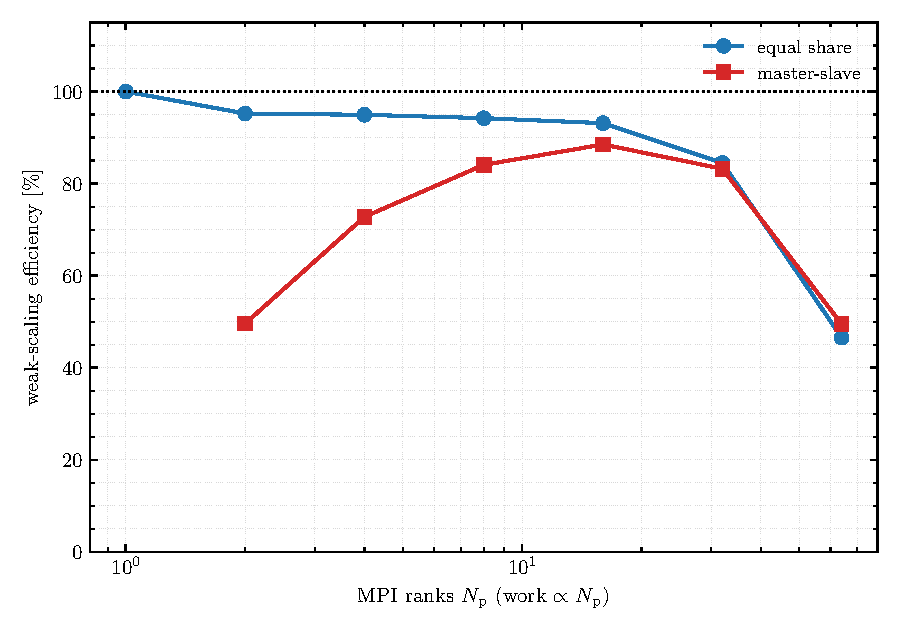
\includegraphics[width=0.72\textwidth]{../examples/scaling/scaling_weak.pdf}
\caption{Weak scaling ($10^{6}$ photons per rank).  Efficiency is
$T_1({\rm eq})/T_{\Np}$.}
\label{fig:weak}
\end{figure}

The flatness of the equal-share curve up to $\Np = 32$ also confirms that the
$J_\lambda$ \code{MPI\_ALLREDUCE} and the output write (both constant in this
series) are negligible at this problem size.  For much larger tallies
($n_\lambda \times n_{\rm cell}$ approaching memory limits) the reduction is
chunked (\file{jtally\_mod}), and its cost should be re-measured together with
the planned tally-memory work.

%=============================================================================
\section{Recommendations}
%=============================================================================
\begin{itemize}
\item \textbf{Do not exceed the physical core count.}  On this node
      $\Np = 32{-}36$ is the sweet spot; hyper-threads add ${\lesssim}5\%$
      throughput while doubling the rank count (and the tally memory, which is
      allocated per rank).
\item \textbf{$\Np \gtrsim 16$: the mode choice hardly matters.}  The
      master--slave penalty is one rank out of $\Np$ and its messaging is free;
      above ${\sim}16$ ranks the two modes agree to a few percent.
\item \textbf{Small $\Np$ (2--8): prefer equal-share} for uniform work such as
      this benchmark --- master--slave wastes 12--50\% of the machine there.
      Use master--slave when the photon cost is strongly nonuniform (deep
      clouds, external illumination, mixed AMR levels), which is why it remains
      the default.
\item \textbf{Oversubscribed or heterogeneous nodes favor master--slave}: its
      dynamic balancing absorbed the hyper-threading nonuniformity at
      $\Np = 64$, beating the static split.
\end{itemize}

%=============================================================================
\section{Reproduction}
%=============================================================================
\begin{itemize}
\item \file{examples/scaling/scale\_base.in} --- the benchmark input.
\item \file{examples/scaling/run\_scaling.sh} --- runs both series and both
      modes, writes \file{results.csv}.
\item \file{examples/scaling/plot\_scaling.py} --- produces
      \file{scaling\_strong.pdf}, \file{scaling\_weak.pdf}, and the rows of
      Table~\ref{tab:strong}.
\end{itemize}

\end{document}
